%document set up stuff
\documentclass[12pt]{article}
\usepackage{helvet}
\usepackage[margin=2.3cm,left=1.5cm,right=1.5cm,bottom=2.4cm]{geometry}
\usepackage{fancyhdr}
\pagestyle{fancy}
\fancyfoot{}
\fancyfoot[R]{ \thepage\ }
\fancyfoot[L]{ Ian McNish }
\usepackage{graphicx}
\usepackage{float}
\usepackage[hidelinks]{hyperref}
\usepackage{listings}
\usepackage{color}
\usepackage{makeidx}
\lstset{
    frame=single,
    breaklines=true,
    postbreak=\raisebox{0ex}[0ex][0ex]{\ensuremath{\color{red}\hookrightarrow\space}}
}
\usepackage[numbers,sort&compress]{natbib}
\usepackage{verbatim}
\usepackage{fancyvrb}
\usepackage{xcolor}
\usepackage{caption}
\usepackage{subcaption}
\usepackage{filecontents}

\newcommand\minput[1]{%
  \input{#1}%
  \ifhmode\ifnum\lastnodetype=11 \unskip\fi\fi}

\usepackage[nottoc,numbib]{tocbibind}

\let\OLDthebibliography\thebibliography
\renewcommand\thebibliography[1]{
  \OLDthebibliography{#1}
  \setlength{\parskip}{0pt}
  \setlength{\itemsep}{0pt plus 0.3ex}
}

\makeindex

\begin{document}

%title page

\begin{titlepage}
\vspace*{2cm}
\begin{center}
\huge{Seed Color ImageJ Manual (unfinished version)}\\
[.75cm]
\large{Ian McNish}\\
\large{University of Minnesota}\\
\large{last modified 22-Feb-2017}
\end{center}

\end{titlepage}

%table of contents

\tableofcontents
%\thispagestyle{empty}
%\cleardoublepage

\thispagestyle{empty}
\cleardoublepage

\pagenumbering{arabic}
\setcounter{page}{1}

%introduction

\section{Introduction}\label{sec:intro}

\noindent This document is meant to serve as a manual for the ImageJ\cite{schneider2012imagej} script  seed\_color\_imagej and R\cite{r} script seed\_color\_r created by Ian McNish. This script was developed to collect color and size data from oat seed samples. This script was originally developed on an Apple MacOS version 10.11 system using Fiji  version 2.0.0. Testing was also completed on a Windows system. In this manual I will explain how this script can be used to analyze seed photos using example photos available on \index{GitHub}. I will also attempt to explain how the script works so that other researchers can modify my code to fit their own needs.

\section{Using ImageJ}\label{sec:imagej}

\subsection{Downloading Fiji}\label{sec:fiji}

\noindent I recommend using Fiji to run this script. Fiji can be found at this website \url{https://fiji.sc}. It is possible to use the script on a vanilla version of ImageJ, but it does require you to separately download the ImageJ macro 'Ellipse Split'. This is easily accomplished using the 'Update' feature in Fiji. Instructions for using using 'Ellipse Split' in ImageJ can be found at \url{http://imagej.net/Ellipse_split}.

\subsection{Downloading tutorial materials from GitHub}\label{sec:github}

\noindent All the materials used in this tutorial can be found at \url{https://github.com/mcnis003/image-analysis/tree/master/seed_color_tutorial}. I will likely develop new versions of this script in the future. The newest version of these scripts can be found at \url{https://github.com/mcnis003/image-analysis.git}.\\

\noindent The materials can be downloaded directly from the \index{GitHub} website. First, navigate to the webpage provided above. Then, select the 'Clone or Download' button on the left side of the page.\\

\begin{figure}[H]
	\centering
	\includegraphics[height=8cm]{/Users/ianmcnish/Documents/imageanalysis/seed_color_scripts/manual/github_web_download_1.png}
	\label{fig:github_web_download_1}
\end{figure}

\noindent Then select the 'Download ZIP' button.

\begin{figure}[H]
	\centering
	\includegraphics[height=8cm]{/Users/ianmcnish/Documents/imageanalysis/seed_color_scripts/manual/github_web_download_2.png}
	\label{fig:github_web_download_2}
\end{figure}

\noindent Alternatively you can also download the files using Terminal commands. A similar system is available on Windows, but I will not supply instructions here. First open \index{Terminal}. I normally do this using the 'Spotlight' feature in MacOS 10.11. You may need to refer to other sources to fully understand Terminal. I will only provide instructions on how to download materials from \index{GitHub} in this manual. While in an appropriate directory use the following commands:\\

\begin{lstlisting}
git clone https://github.com/mcnis003/image-analysis.git
\end{lstlisting}

\begin{figure}[H]
	\centering
	\includegraphics[height=8cm]{/Users/ianmcnish/Documents/imageanalysis/seed_color_scripts/manual/github_terminal_download_1.png}
	\label{fig:github_terminal_download_1}
\end{figure}


\subsection{Downloading Ellipse Split}\label{sec:ellipse_split}

\noindent Downloading `\index{Ellipse Split}' is easiest when using Fiji. `Ellipse Split' works in vanilla ImageJ but the installation process is slightly more calculated. I will not provide instructions for downloading `Ellipse Split' for use in vanilla ImageJ. 

\begin{enumerate}

\item To download `Ellipse Split', navigate the the Fiji `Help' menu and select `Update...'\\

\begin{figure}[H]
	\centering
	\includegraphics[height=8cm]{/Users/ianmcnish/Documents/imageanalysis/seed_color_scripts/manual/ellipse_split_download_1.png}
	\label{fig:ellipse_split_download_1}
\end{figure}

\item After Fiji has completed updating press `OK'. Then select `Manage update sites'.\\

\begin{figure}[H]
	\centering
	\includegraphics[height=8cm]{/Users/ianmcnish/Documents/imageanalysis/seed_color_scripts/manual/ellipse_split_download_2.png}
	\label{fig:ellipse_split_download_2}
\end{figure}

\item Select `\index{Biomedgroup}' from the list and select `Add update site'. `\index{Ellipse Split}' should then be available in you `Macro' menu.\\

\begin{figure}[H]
	\centering
	\includegraphics[height=8cm]{/Users/ianmcnish/Documents/imageanalysis/seed_color_scripts/manual/ellipse_split_download_3.png}
	\label{fig:ellipse_split_download_3}
\end{figure}

\end{enumerate}

\subsection{Open the script}\label{sec:open_script}

\noindent Now that we have Fiji, Ellipse Split, and the materials from \index{GitHub} downloaded we are ready to open the script in \index{Fiji}. Do this through the open command in Fiji.\\

\begin{enumerate}

\item Select `Open' in the `File' menu.\\

\begin{figure}[H]
	\centering
	\includegraphics[height=8cm]{/Users/ianmcnish/Documents/imageanalysis/seed_color_scripts/manual/open_imagej_script_1.png}
	\label{fig:open_imagej_script_1}
\end{figure}

\item Select the script you wish to open.\\

\begin{figure}[H]
	\centering
	\includegraphics[height=8cm]{/Users/ianmcnish/Documents/imageanalysis/seed_color_scripts/manual/open_imagej_script_2.png}
	\label{fig:open_imagej_script_2}
\end{figure}

\item The script will then open in \index{Fiji}'s editing environment. The entire script may be run using the 'Run' button or by pressing `command'+`R' on Mac. To run a portion of the code select the lines you wish to run a press `command'+`shift'+`R'.\\

\begin{figure}[H]
	\centering
	\includegraphics[height=8cm]{/Users/ianmcnish/Documents/imageanalysis/seed_color_scripts/manual/open_imagej_script_3.png}
	\label{fig:open_imagej_script_3}
\end{figure}

\item Finally, the language of the script must be selected. Choose `IJ1 Macro' from the `Language' menu.\\

\begin{figure}[H]
	\centering
	\includegraphics[height=8cm]{/Users/ianmcnish/Documents/imageanalysis/seed_color_scripts/manual/open_imagej_script_4.png}
	\label{fig:open_imagej_script_3}
\end{figure}

\end{enumerate}

\subsection{Setting parameters in ImageJ}\label{sec:parameters}

\noindent Parameters other than the file directory should not need to be changed to run the Tutorial photos available on \index{GitHub}. However, you will definitely need to change the parameters for photos you collect. The script works by dividing the image into separate zones. Each zone contains elements that are used for different processes. The position of the zones will depend on how you arrange your items in the photo, the equipment you use to take the photo, and the settings of your equipment. I suggest you test a couple different arrangements, and then strictly stick to the arrangement you think is most optimal.\\

\subsubsection{Using cleanup mode}

\noindent The cleanup variable can be set to eiter `true' or `false'. Cleanup mode is enabled when the cleanup variable equals `true'. This script creates many intermediate files when processing photos. These files can occupy a large amount of space. When cleanup mode is enabled, the script will delete many of these files. The only files that will not be deleted are the original photo files and the data result files. As a safety precaution the delete function in ImageJ will only function if the file pathway includes a directory named ``ImageJ". Cleanup mode is probably not useful when you are first learning to use the script, or when you a troubleshooting.\\

\begin{figure}[H]
	\centering
	\includegraphics[height=8cm]{/Users/ianmcnish/Documents/imageanalysis/seed_color_scripts/manual/imagej_cleanup_mode.png}
	\label{fig:open_imagej_script_3}
\end{figure}

\subsubsection{Choosing the file pathway}\label{sec:pathway}

\noindent You will need to change the directory defined on line 45 of the script to the directory containing your photos. The result files will also be written to this directory. The behavior of this part of the script is similar to the setwd() command in R.\\

\begin{figure}[H]
	\centering
	\includegraphics[height=8cm]{/Users/ianmcnish/Documents/imageanalysis/seed_color_scripts/manual/imagej_change_file_directory.png}
	\label{fig:imagej_change_file_directory}
\end{figure}

\subsubsection{Enter control patch coordinates}\label{sec:control_patch_coords}

\noindent The coordinate of you control patches must be entered in this part of the script. These must be entered as an array because each point in the array is specifically referenced later in the script. If you use more or less control patches you will need to modify this section and the calibration sections later in the script. You will need to determine if your application requires \index{radiometric calibration}.\\

\begin{figure}[H]
	\centering
	\includegraphics[height=8cm]{/Users/ianmcnish/Documents/imageanalysis/seed_color_scripts/manual/imagej_control_patch_coords.png}
	\label{fig:imagej_control_patch_coords}
\end{figure}

\subsubsection{Enter seed coordinates}\label{sec:seed_coords}

\noindent Enter the coordinates of the seeds here. Seeds that are on the edge of the region you draw will not be included in the analysis if you use `\index{Ellipse Split}' with the default settings from my script.\\

\begin{figure}[H]
	\centering
	\includegraphics[height=8cm]{/Users/ianmcnish/Documents/imageanalysis/seed_color_scripts/manual/imagej_seed_coords.png}
	\label{fig:imagej_change_file_directory}
\end{figure}

\subsubsection{Enter control patch reflectance data}\label{sec:control_patch_reflectance}

\noindent Enter the control patch expected reflectance data here. You will need to do this three times (lines 152, 193, and 227).\\

\begin{figure}[H]
	\centering
	\includegraphics[height=8cm]{/Users/ianmcnish/Documents/imageanalysis/seed_color_scripts/manual/imagej_control_patch_parameters.png}
	\label{fig:imagej_control_patch_parameters}
\end{figure}

\subsubsection{Changing initial photo file type}\label{sec:file_type}

\noindent The Tutorial variable uses the .jpg file type to match the photos available on GitHub. The script has also been tested with TIFF format photos. You will need to change the extension here to match the type of photos you use here.\\

\begin{figure}[H]
	\centering
	\includegraphics[height=8cm]{/Users/ianmcnish/Documents/imageanalysis/seed_color_scripts/manual/imagej_photo_file_type.png}
	\label{fig:imagej_photo_file_type}
\end{figure}

\section{Running the script in Fiji}\label{sec:run_imagej_script}

\noindent Once all your parameters are set you can run the script by pressing the `Run' button in the development window or by pressing `command'+'R' on Mac.\\

\begin{figure}[H]
	\centering
	\includegraphics[height=8cm]{/Users/ianmcnish/Documents/imageanalysis/seed_color_scripts/manual/imagej_run_script.png}
	\label{fig:imagej_run_script}
\end{figure}

\section{Using R}\label{sec:r}

\begin{figure}[H]
	\centering
	\includegraphics[height=8cm]{/Users/ianmcnish/Documents/imageanalysis/seed_color_scripts/manual/r_set_working_directory.png}
	\label{fig:r_set_working_directory}
\end{figure}

\section{Tips for taking photos}\label{sec:photos}

enter information about using this script

\section{ImageJ process walkthrough}\label{sec:imagej_process}

enter information about using this script

\subsection{Section 3: importing the photo and splitting channels}\label{sec:imagej_import_split}

\begin{enumerate}

\item The full color photo is opened.\\

\begin{figure}[H]
	\centering
	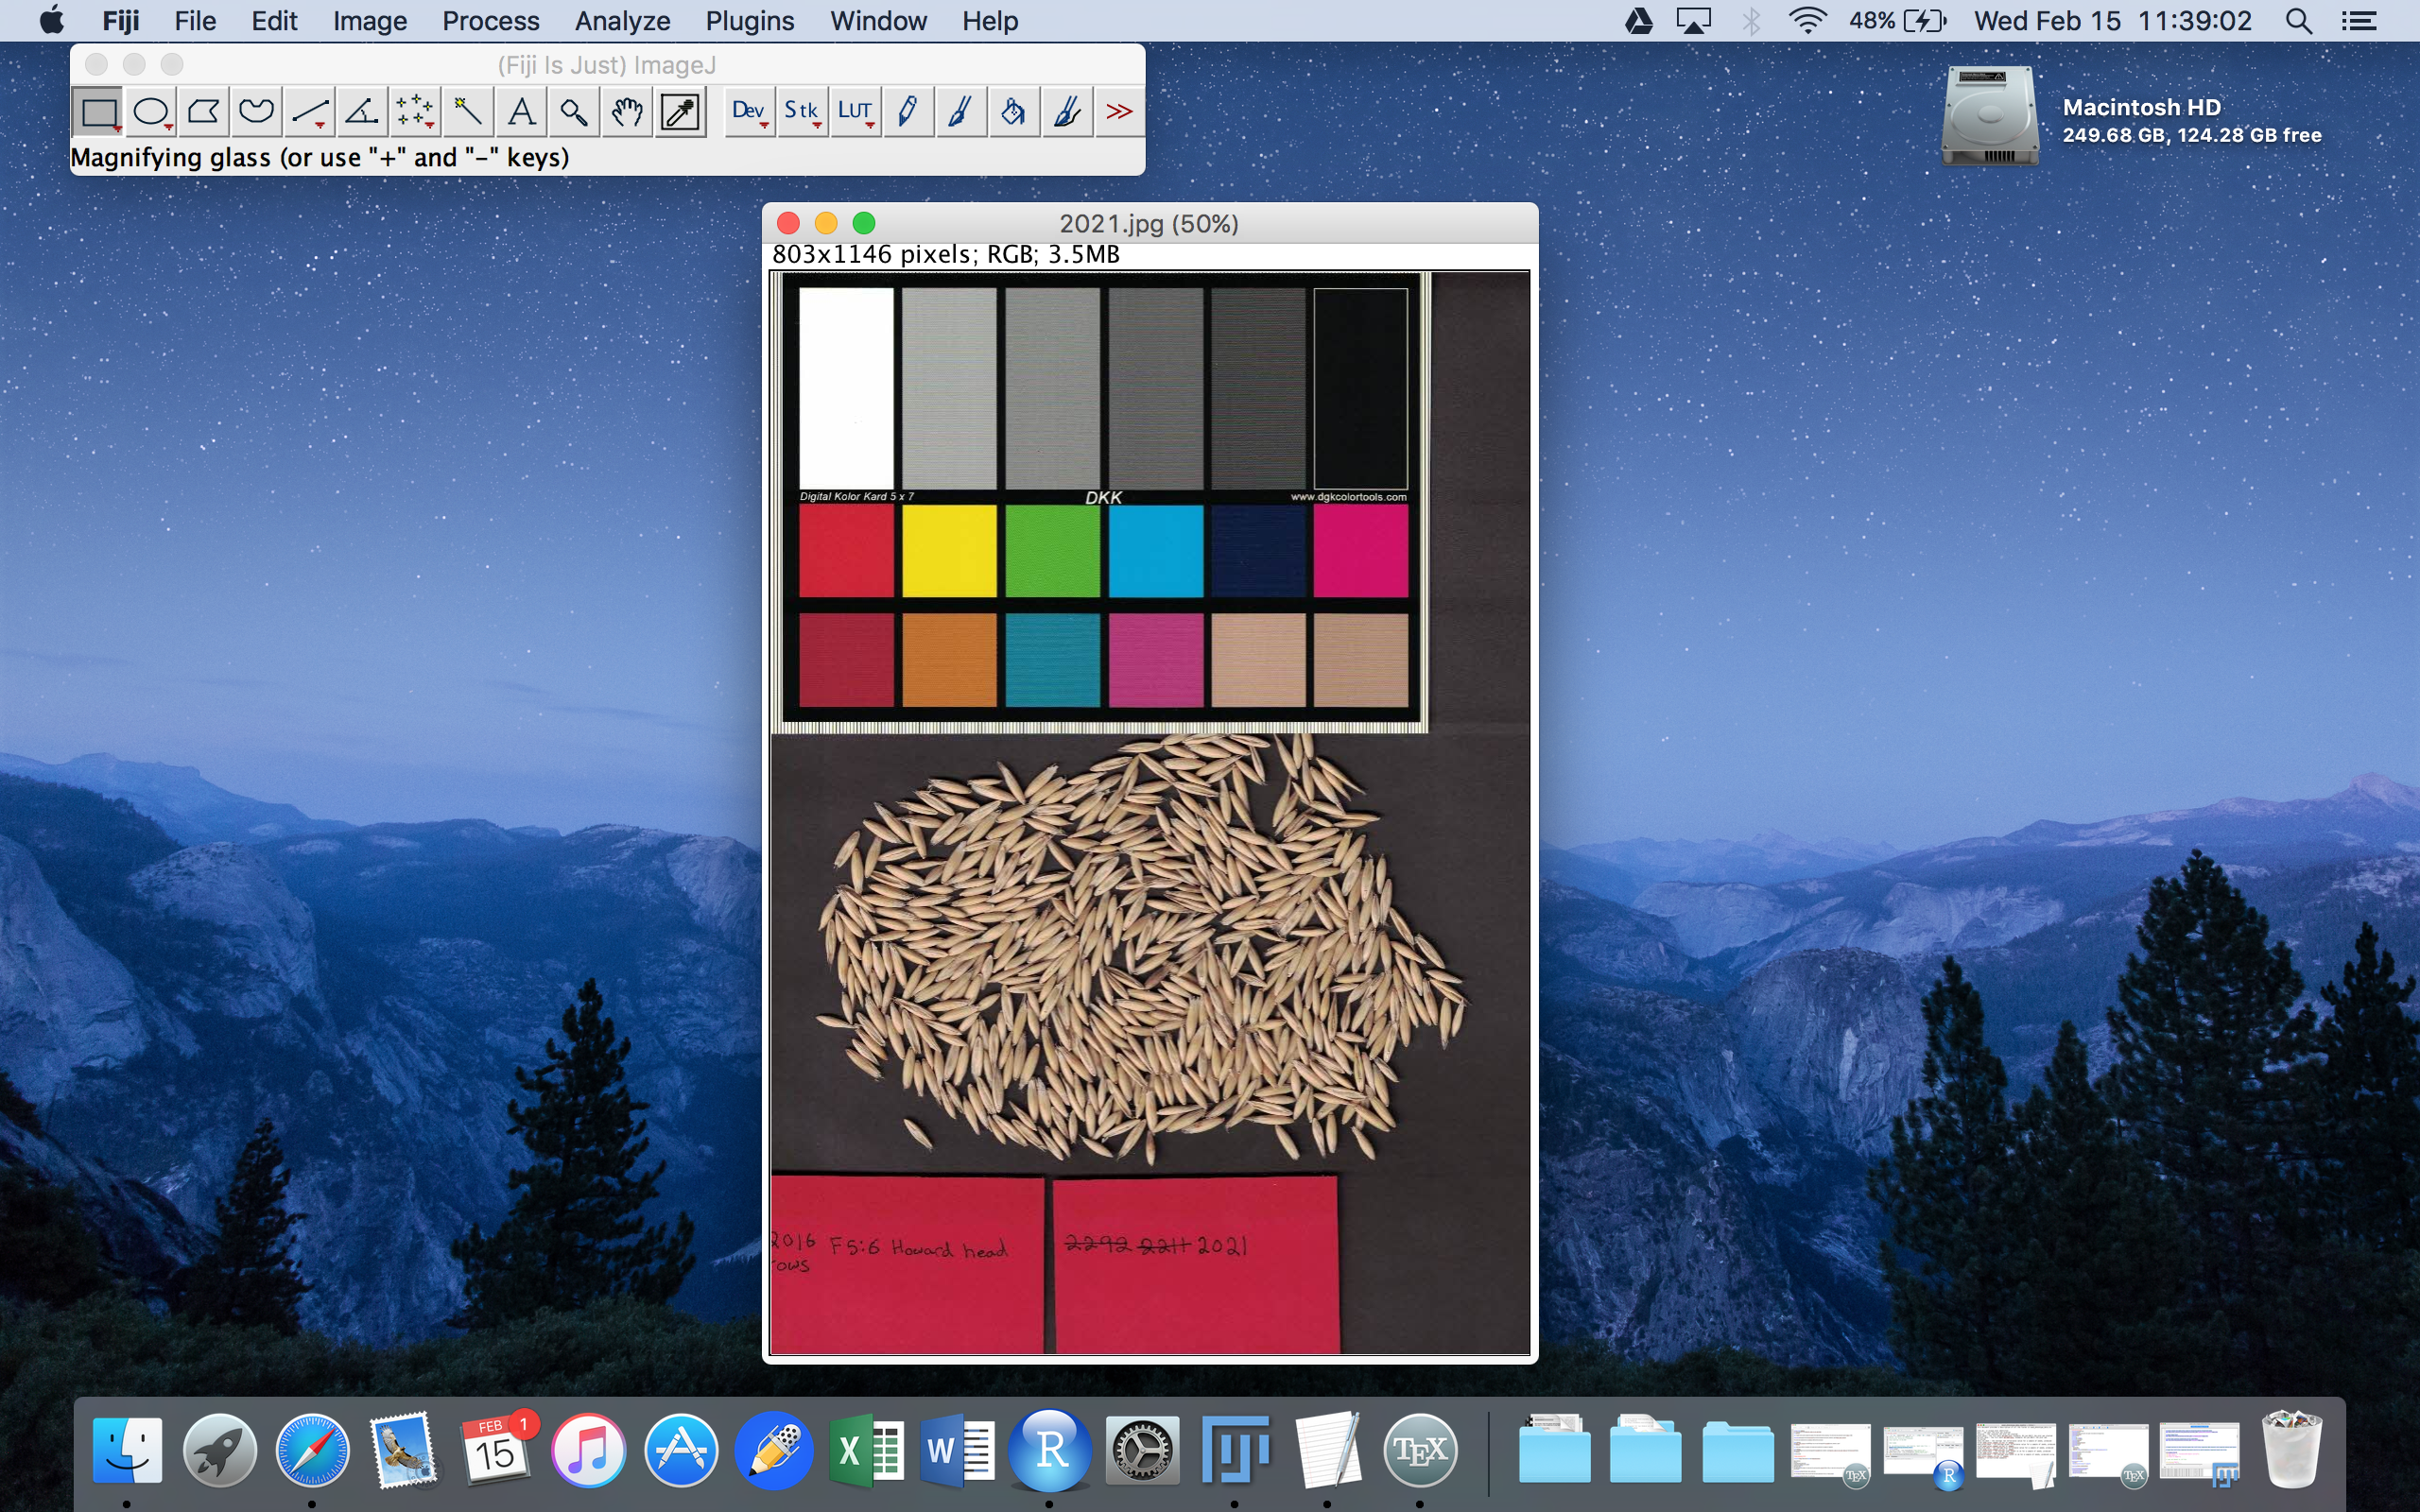
\includegraphics[height=8cm]{/Users/ianmcnish/Documents/imageanalysis/seed_color_scripts/manual/imagej_open_image.png}
	\label{fig:imagej_open_image}
\end{figure}

\item The photo is then split into R, G, and B channels in a stack.\\

\begin{figure}[H]
	\centering
	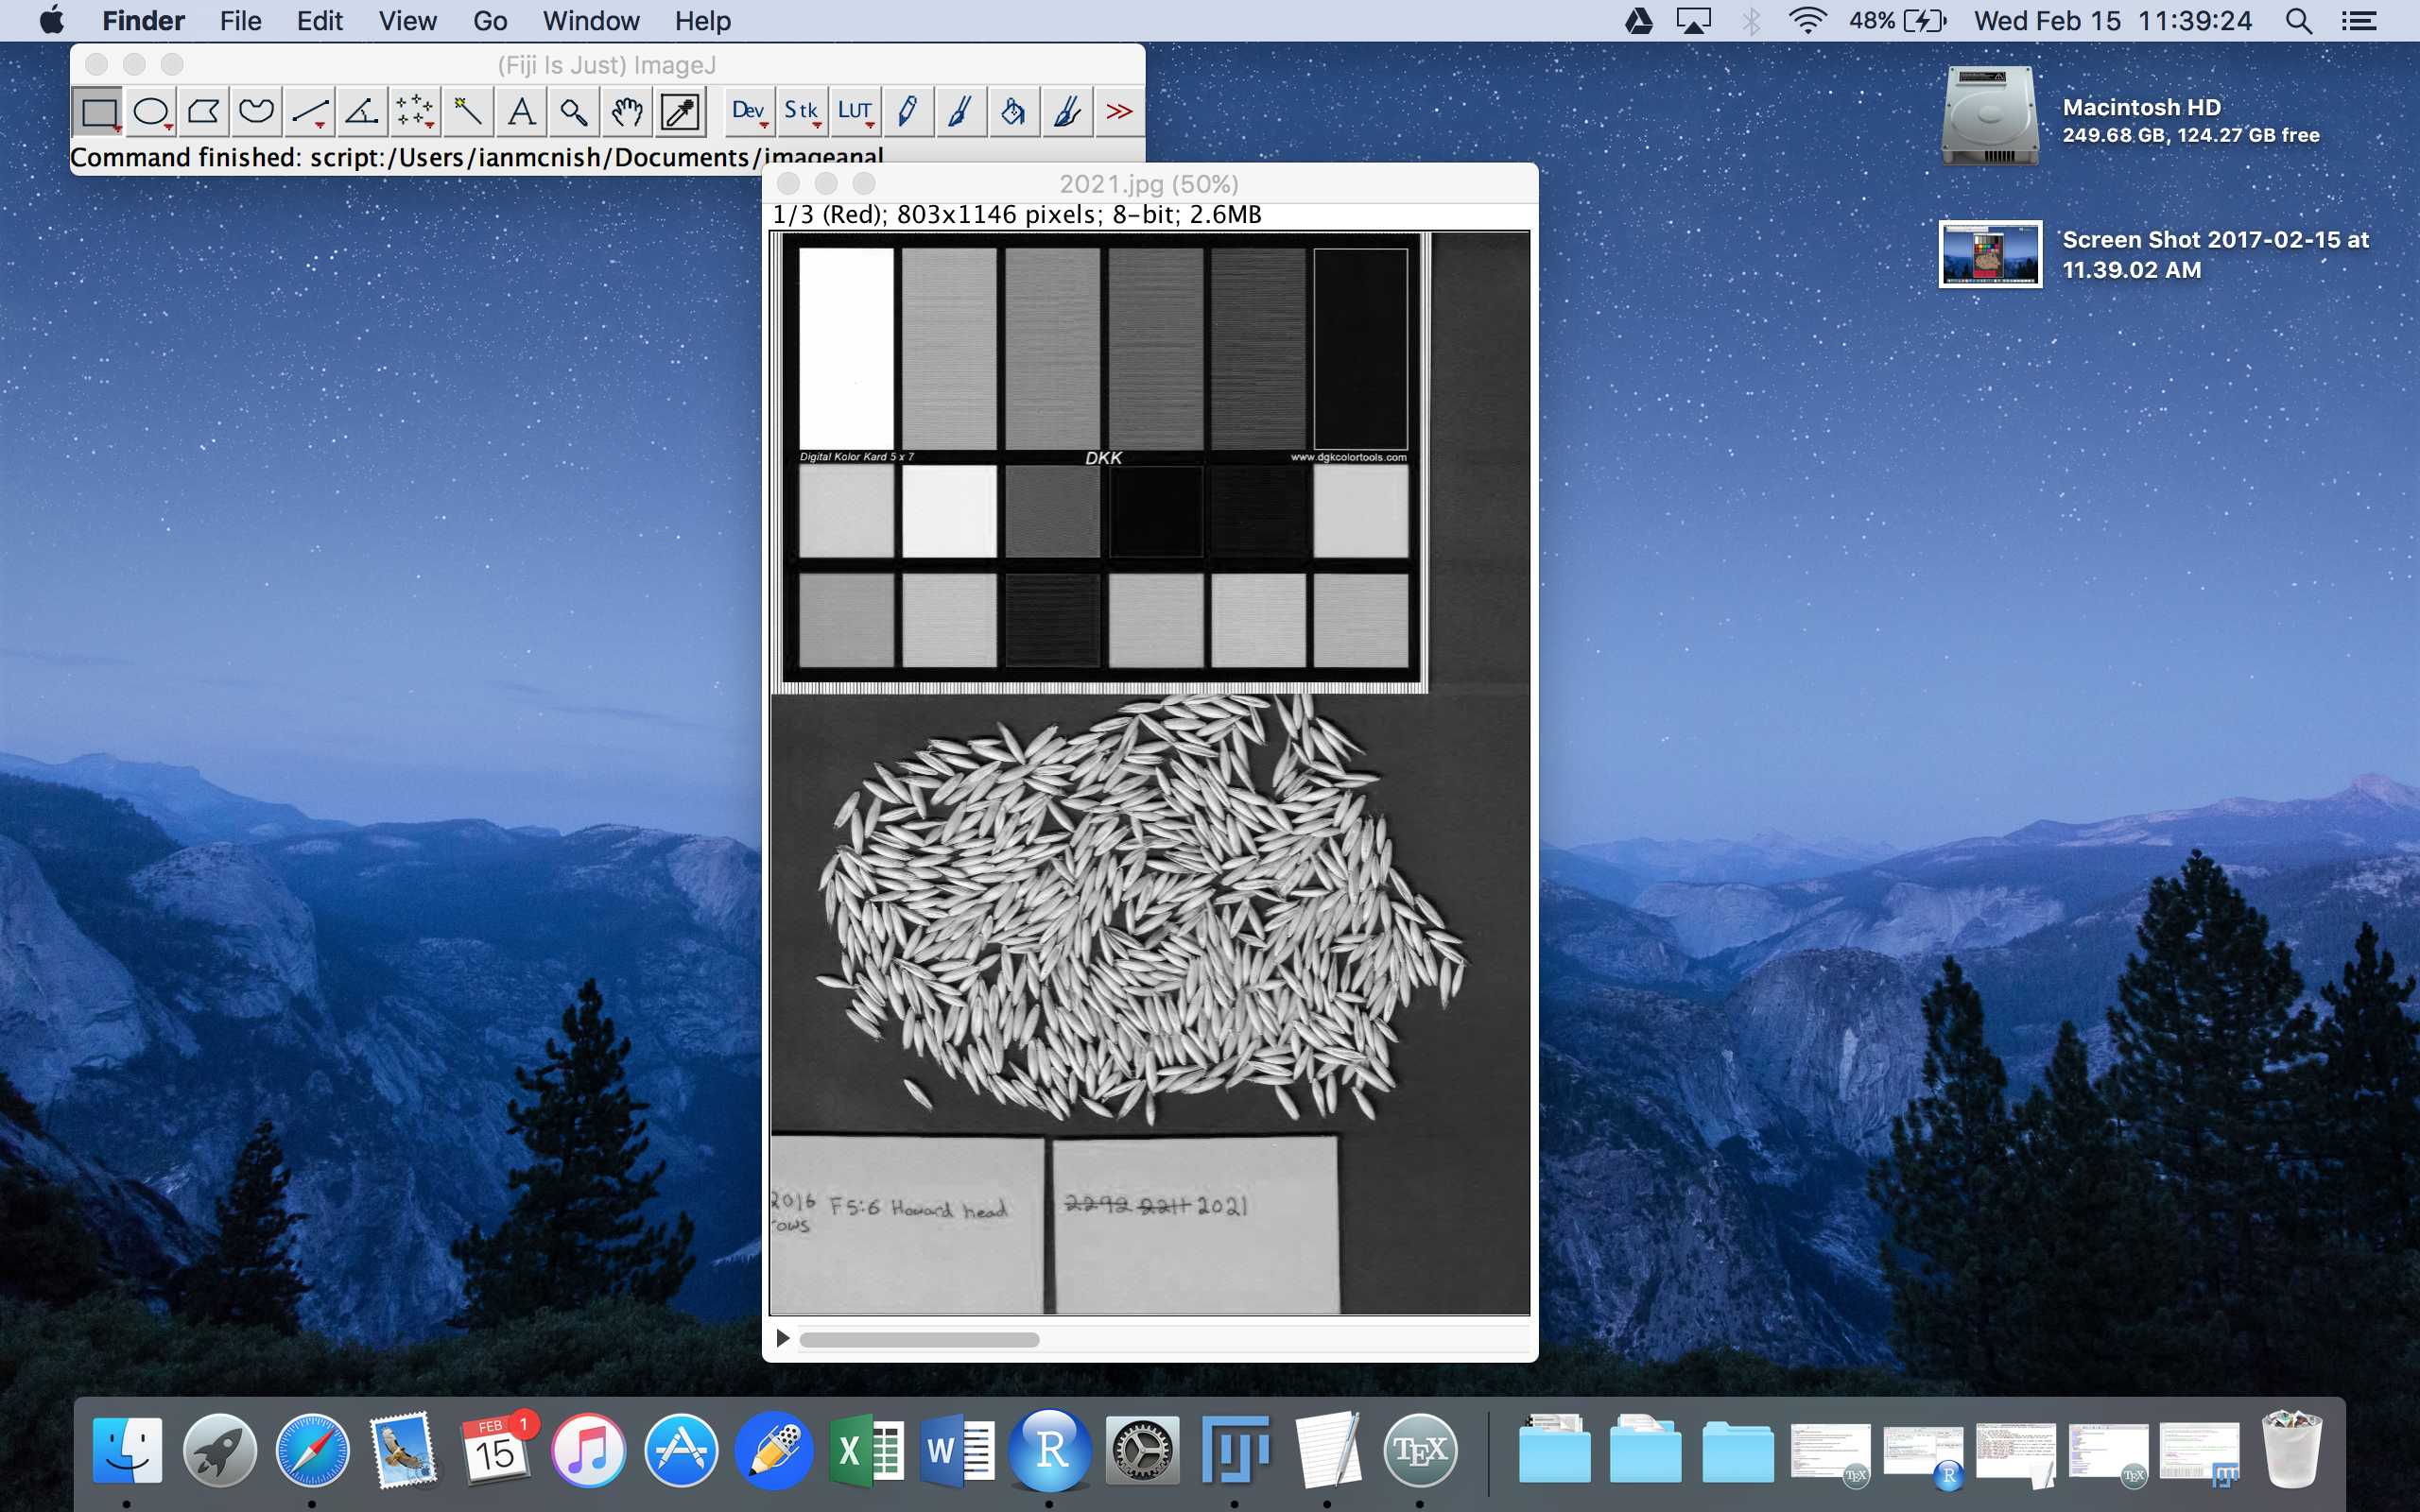
\includegraphics[height=8cm]{/Users/ianmcnish/Documents/imageanalysis/seed_color_scripts/manual/imagej_split_channels.png}
	\label{fig:imagej_split_channels}
\end{figure}

\item The stack of channels is then split into separate photos and each photo is saved. All photos are saved in TIFF format from this point onwards.\\

\begin{figure}[H]
	\centering
	\includegraphics[height=8cm]{/Users/ianmcnish/Documents/imageanalysis/seed_color_scripts/manual/imagej_separate_stack.png}
	\label{fig:imagej_separate_stack}
\end{figure}

\end{enumerate}

\subsection{Section 4: radiometric calibration}\label{sec:imagej_radiometrics_calibration}

\noindent Radiometric calibration is accomplished using a standard photo card placed in each photo combined with data collected with sensitive laboratory equipment. A detailed explanation of this method is provided by \url{http://ieeexplore.ieee.org/document/7098353/?reload=true}. Ultimately you will need to decide if you need to calibrate your photos. Radiometric calibration should be less important in circumstances with very controlled image acquisition. I provided the code in this script so that other researchers could use it if it is important in their process.\\

\begin{figure}[H]
	\centering
	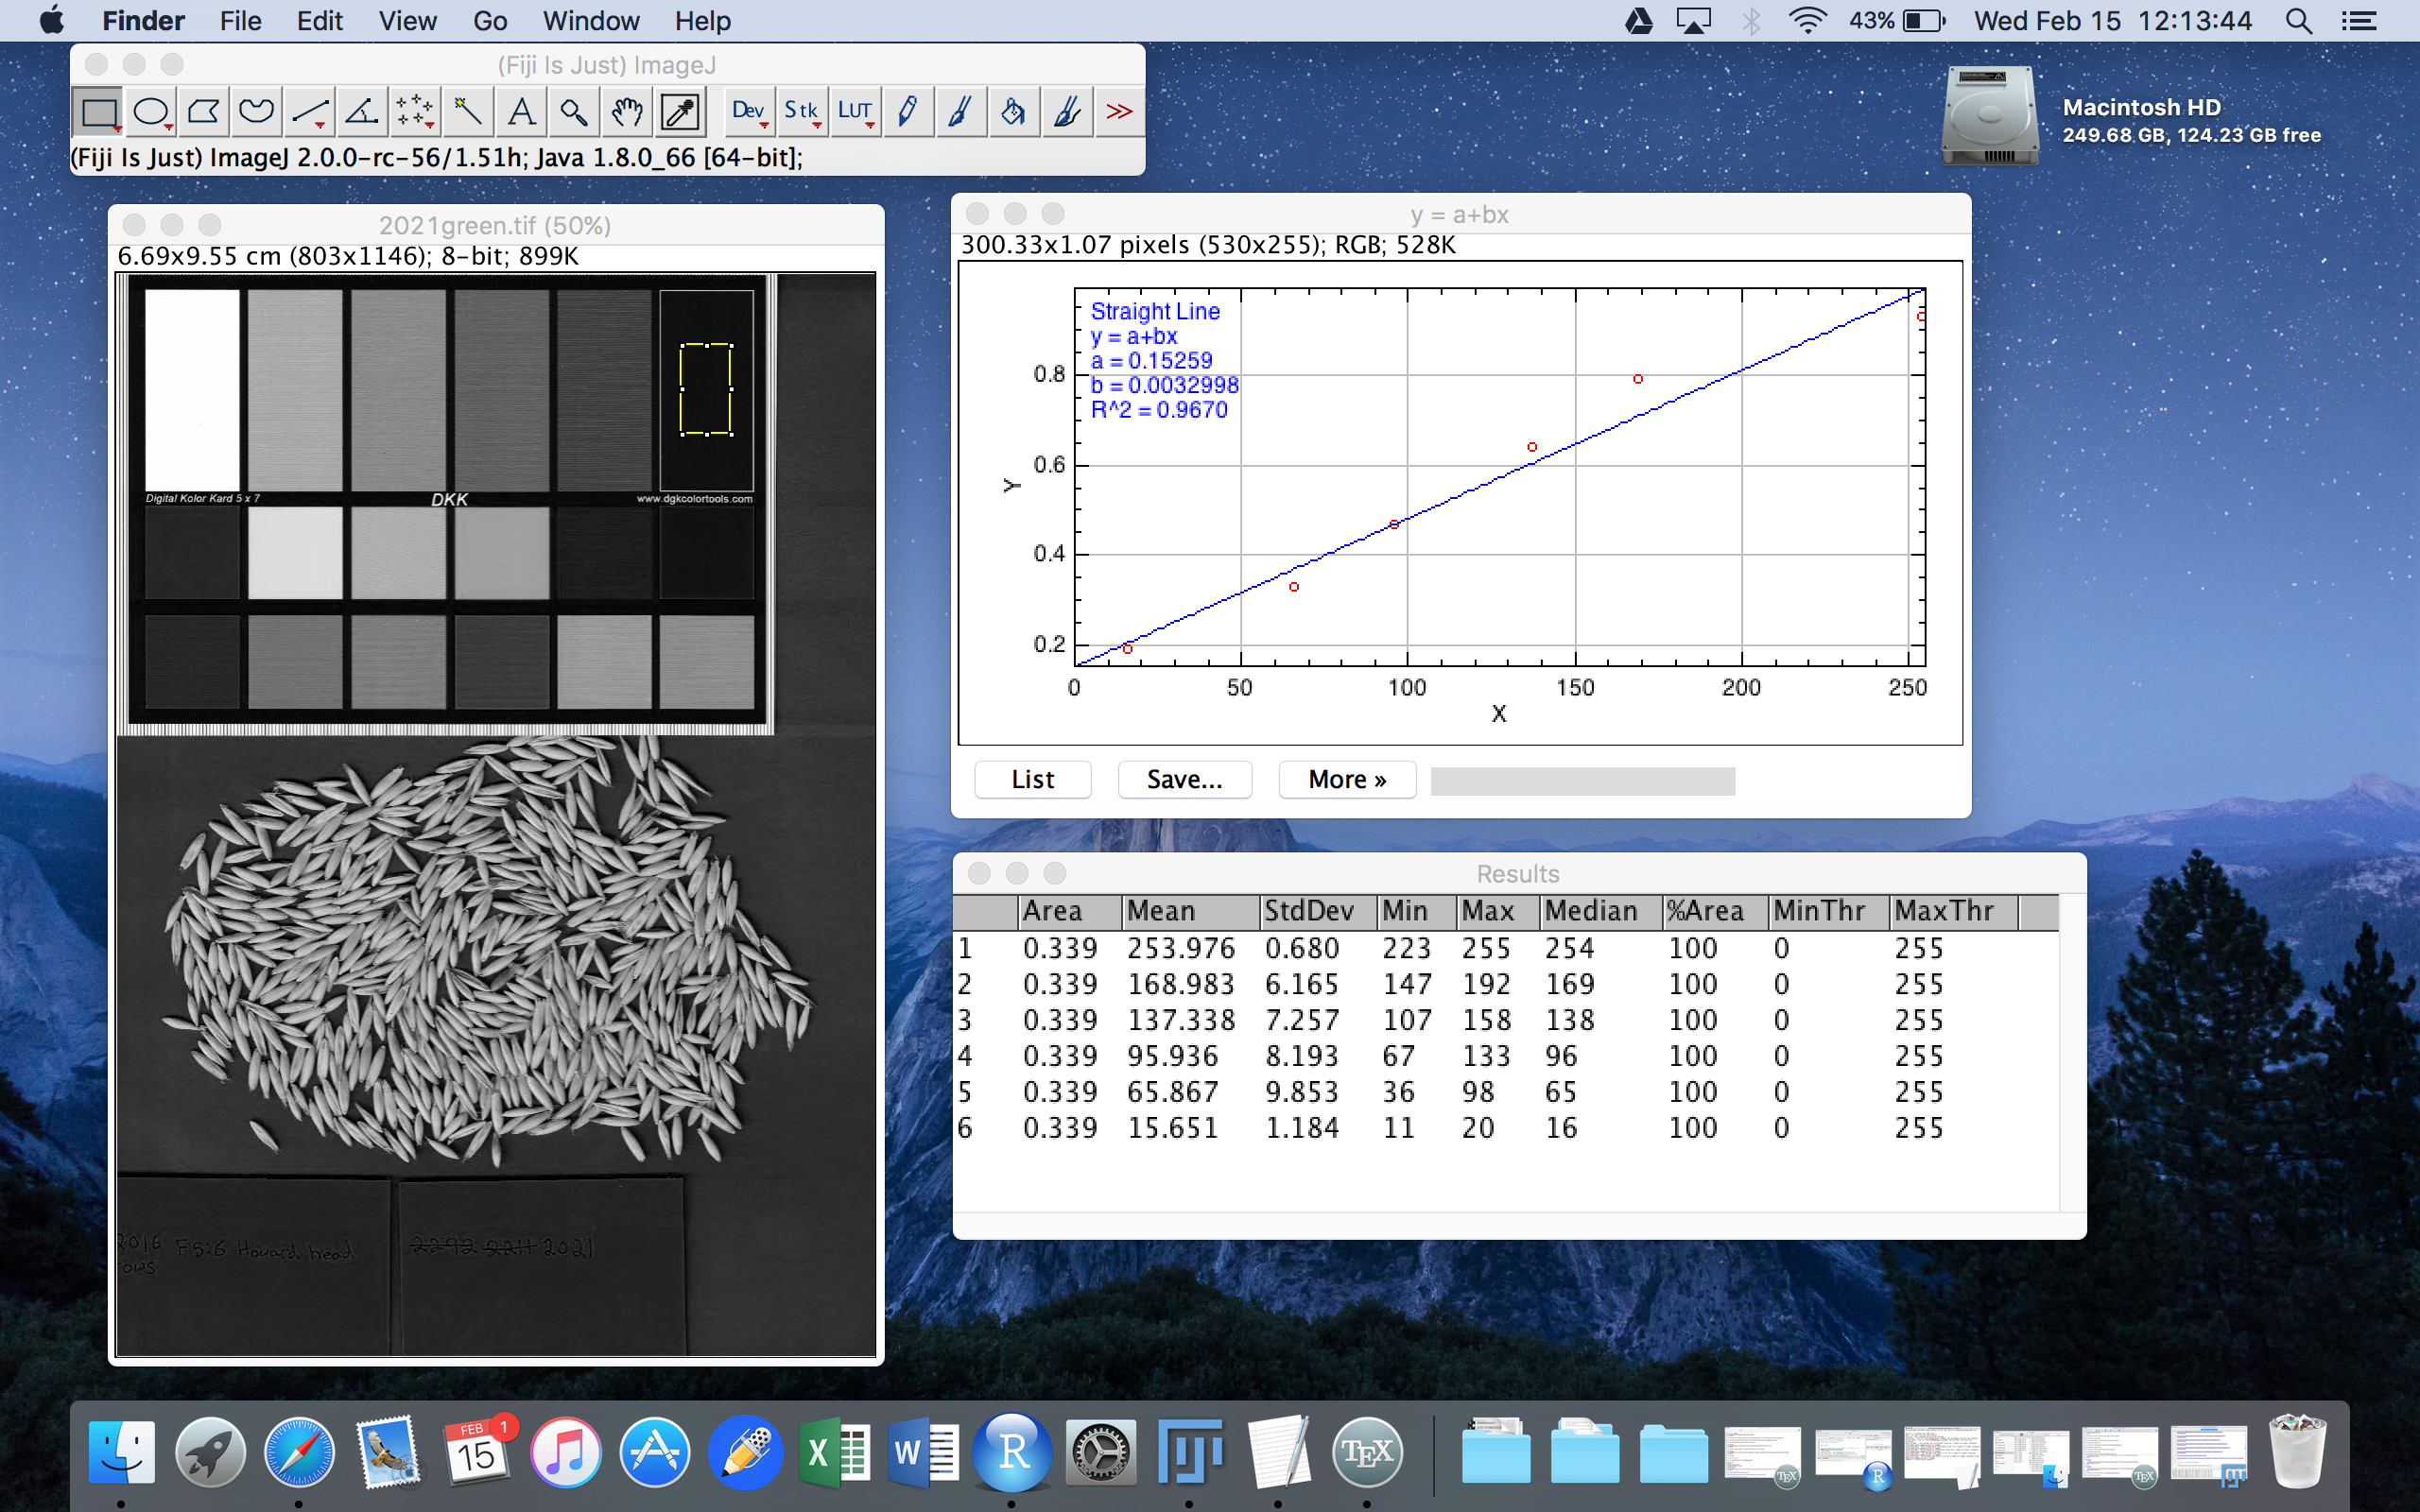
\includegraphics[height=8cm]{/Users/ianmcnish/Documents/imageanalysis/seed_color_scripts/manual/imagej_radiometric_calibration.png}
	\label{fig:imagej_radiometric_calibration}
\end{figure}

\subsection{Section 6: background masking}\label{sec:imagej_background_masking}

\noindent For our application, background masking was not required. However, the mask is used by `Ellipse Split' to produce the seed ROIs. I also use color data collected from the mask file to find instances where a seed ROI contains multiple seeds or large amounts of background. Masking may be necessary if your background is irregular.\\

\begin{figure}[H]
	\centering
	\includegraphics[height=8cm]{/Users/ianmcnish/Documents/imageanalysis/seed_color_scripts/manual/imagej_mask.png}
	\label{fig:imagej_mask}
\end{figure}

\subsection{Section 7: using Ellipse Split to create seed ROIs}\label{sec:imagej_ellipse_split}

\noindent Because our seeds are ellipse shaped, I used the ImageJ macro `\index{Ellipse Split}' to find ROIs. If you are analyzing objects of another shape this method of locating the object will probably not work. For other shapes of object I recommend using the `\index{Analyze Particles}'  command.\\

\begin{figure}[H]
	\centering
	\includegraphics[height=8cm]{/Users/ianmcnish/Documents/imageanalysis/seed_color_scripts/manual/imagej_seeds_identified.png}
	\label{fig:imagej_seeds_identified}
\end{figure}

\section{FAQ}\label{sec:faq}

\begin{enumerate}

\item Q: how long does it take to analyze a photo with this program?\\
\noindent A: Our application uses a ~30mb photo with ~100 objects and it takes ~4 seconds per photo. The program is much faster if batch mode is enabled, but unfortunately I have been having problems with batch mode lately.

\item Q: How accurate is the script at finding seeds?
A: In our experience, if items in the photo are well arranged the script will accurately find ~85\% of the seeds, 5\% of the seeds will be misidentified in some way, and 10\% of the seeds will not be identified.

\end{enumerate}

\bibliographystyle{acm}
\bibliography{/Users/ianmcnish/Documents/combinedbibliography.bib}

\printindex

\end{document}
